\documentclass[12pt,letterpaper]{article}
\usepackage[utf8]{inputenc}
\usepackage[spanish]{babel}
\usepackage{graphicx}
\usepackage[left=2cm,right=2cm,top=2cm,bottom=2cm]{geometry}
\usepackage{graphicx} % figuras
% \usepackage{subfigure} % subfiguras
\usepackage{float} % para usar [H]
\usepackage{amsmath}
%\usepackage{txfonts}
\usepackage{stackrel} 
\usepackage{multirow}
\usepackage{enumerate} % enumerados
\renewcommand{\labelitemi}{$-$}
\renewcommand{\labelitemii}{$\cdot$}
% \author{}
% \title{Caratula}
\begin{document}

% Fancy Header and Footer
% \usepackage{fancyhdr}
% \pagestyle{fancy}
% \cfoot{}
% \rfoot{\thepage}
%

% \usepackage[hidelinks]{hyperref} % CREA HYPERVINCULOS EN INDICE

% \author{}
\title{Caratula}

\begin{titlepage}
\begin{center}
\large{UNERSIDAD PRIVADA DE TACNA}\\
\vspace*{-0.025in}
\begin{figure}[htb]
\begin{center}

\includegraphics[width=8cm]{./Imagenes/logo}
\end{center}
\end{figure}
\vspace*{0.15in}
ESCUELA PROFESIONAL DE INGENIERIA DE SISTEMAS  \\

\vspace*{0.5in}
\begin{large}
TITULO:\\
\end{large}

\vspace*{0.1in}
\begin{Large}
\textbf{INFORME DE LABORATORIO No 01} \\
\end{Large}

\vspace*{0.3in}
\begin{Large}
\textbf{CURSO:} \\
\end{Large}

\vspace*{0.1in}
\begin{large}
INTELIGENCIA DE NEGOCIOS\\
\end{large}

\vspace*{0.3in}
\begin{Large}
\textbf{DOCENTE(ING):} \\
\end{Large}

\vspace*{0.1in}
\begin{large}
 Patrick Cuadros Quiroga\\
\end{large}

\vspace*{0.2in}
\vspace*{0.1in}
\begin{large}
Alumno: \\
\begin{flushleft}
Guimer Senon Coaquira Coaquira	\hfill	(2015053226) \\
\end{flushleft}
\end{large}
\end{center}

\end{titlepage}


\tableofcontents % INDICE
\thispagestyle{empty} % INDICE SIN NUMERO
\newpage
\setcounter{page}{1} % REINICIAR CONTADOR DE PAGINAS DESPUES DEL INDICE
\begin{center}
\vspace*{0.1in}
\begin{Large}
\textbf{PRACTICA DE LABORATORIO N° 01:} \\
\textbf{(Elaboración de Dashboards en Power BI)} \\
\end{Large}
\end{center}
\begin{document}
\section{OBJETIVO:}
\item{
Desarrollar el Informe de Labratorio 01 de Dashboards en Power BI}
\section{REQUERIMIENTOS}
\item{Conocimientos
Para el desarrollo de esta práctica se requerirá de los siguientes conocimientos básicos:\\
- Conocimientos básicos de administración de base de datos Microsoft SQL Server.\\
- Conocimientos básicos de SQL.\\
✓ Software
Asimismo se necesita los siguientes aplicativos:
- Microsoft SQL Server 2016 o superior\\
- Base de datos AdventureWorks2016 o superior\\
- Power BI Desktop.\\
- Tener una cuenta Microsoft registrada en el Portal de Power Bi}\\

\section{CONSIDERACIONES INICIALES}
\item{Generar una carpeta o directorio Power BI en un lugar accesible para guardar los resultados de la práctica.}\\
\\\\\\\\\\\\\\\\\\\\\\\\\\\\
\section{DESARROLLO}

\subsection{RESULTADO Nº01:}
\begin{figure}[httb]
\begin{center}
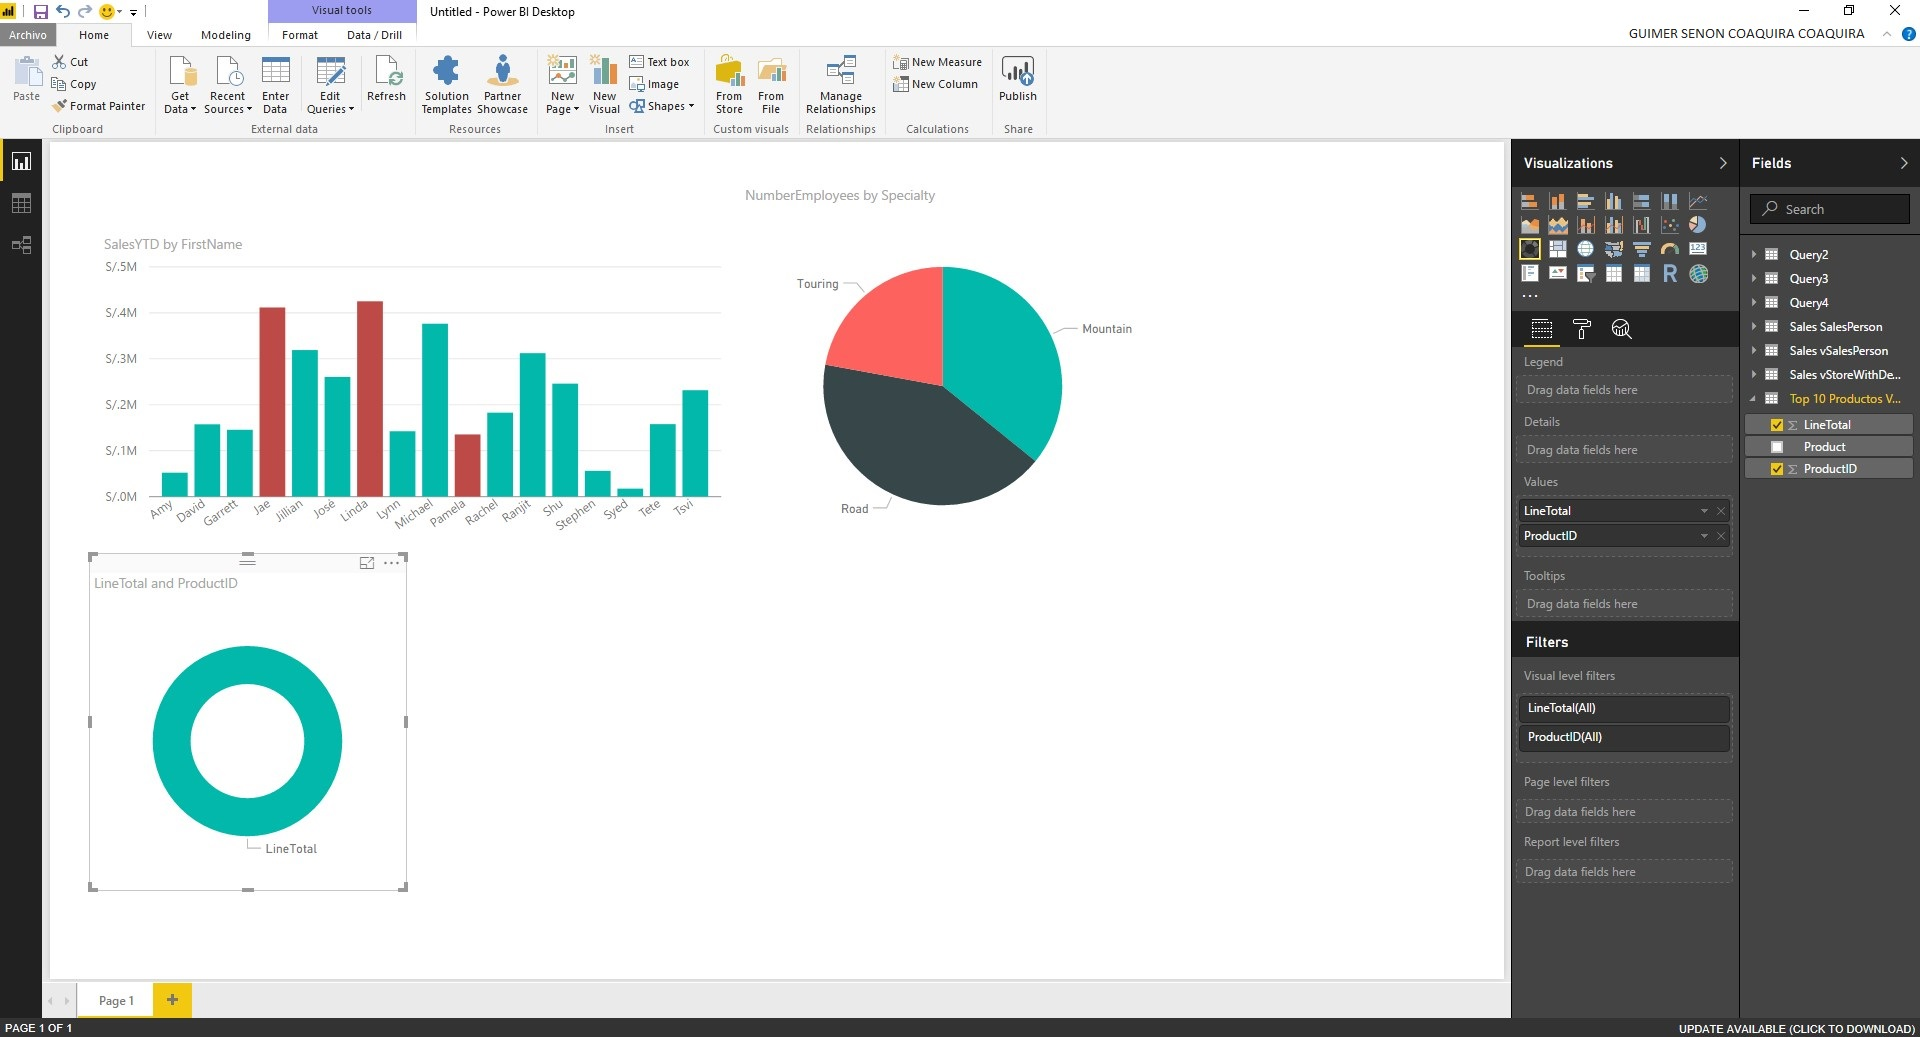
\includegraphics[width=15cm]{./Imagenes/Captura01}
\end{center}
\end{figure}

\subsection{RESULTADO Nº02:}
\begin{figure}[httb]
\begin{center}
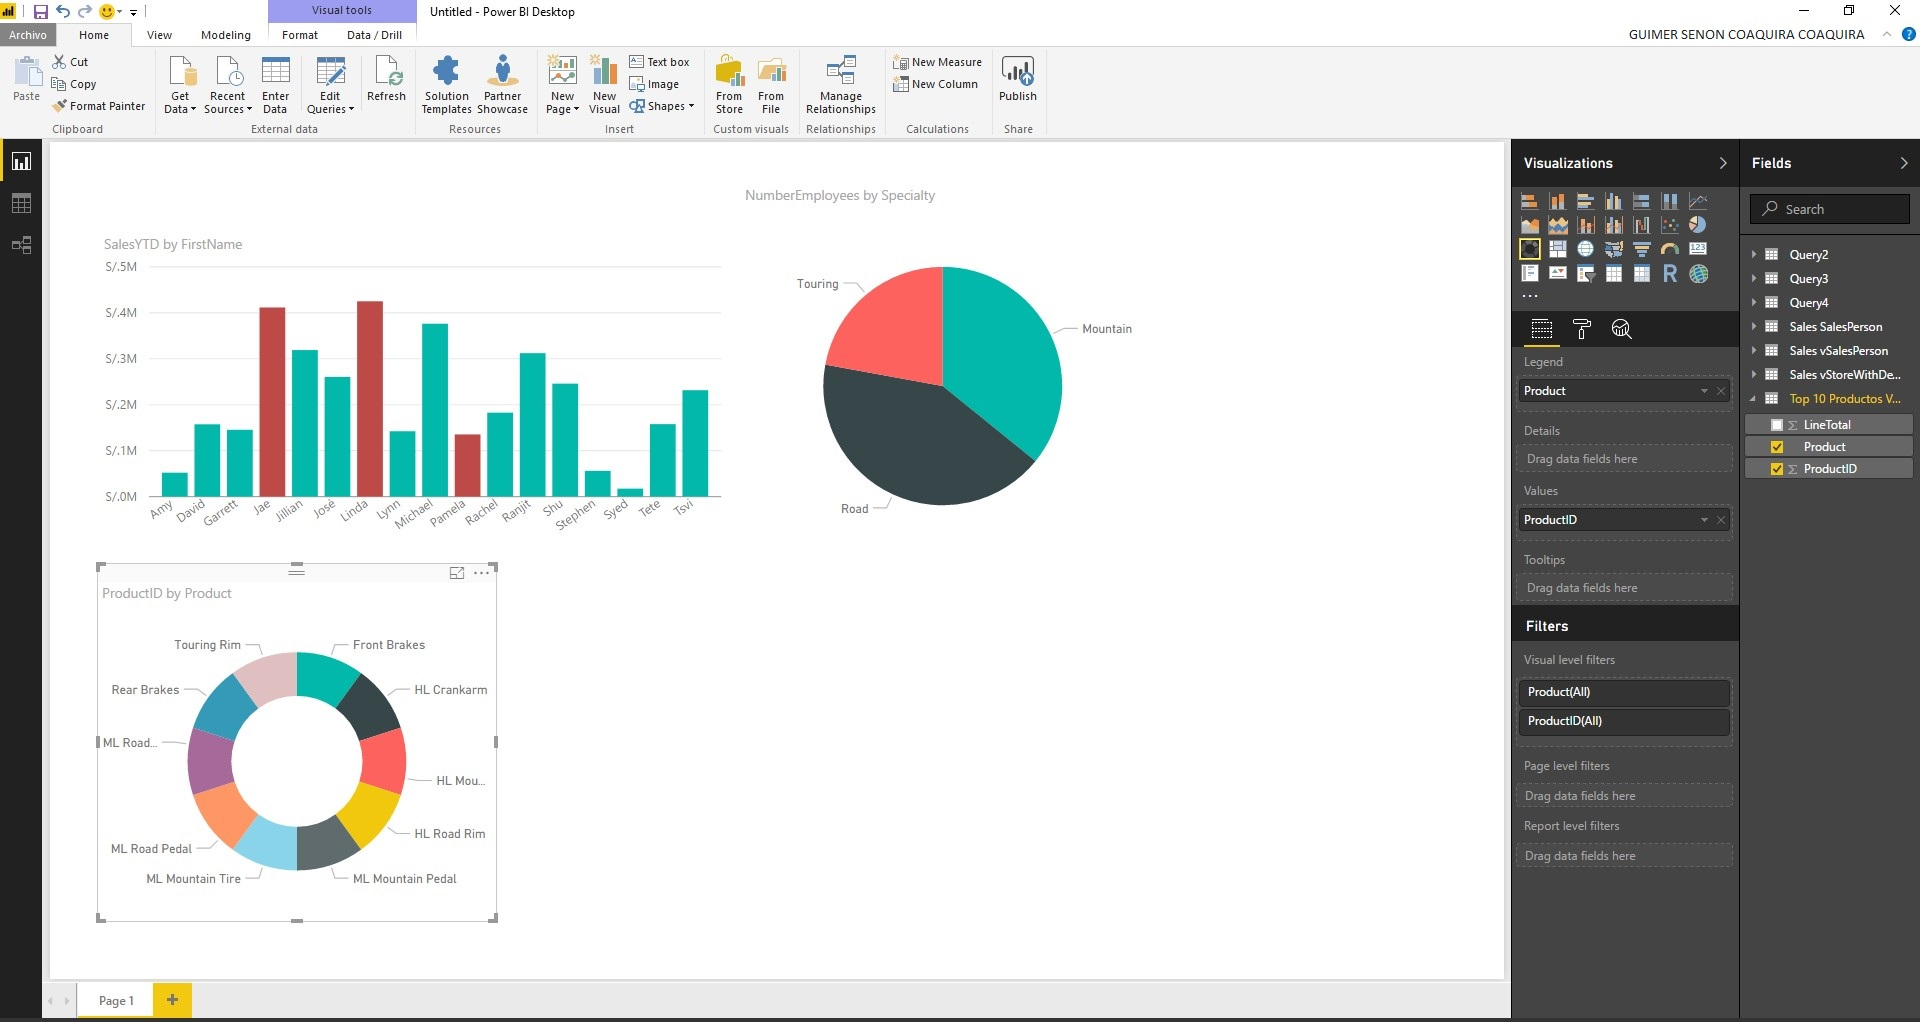
\includegraphics[width=15cm]{./Imagenes/Captura02}
\end{center}
\end{figure}
\newpage
\subsection{RESULTADO Nº03:}
\begin{figure}[httb]
\begin{center}
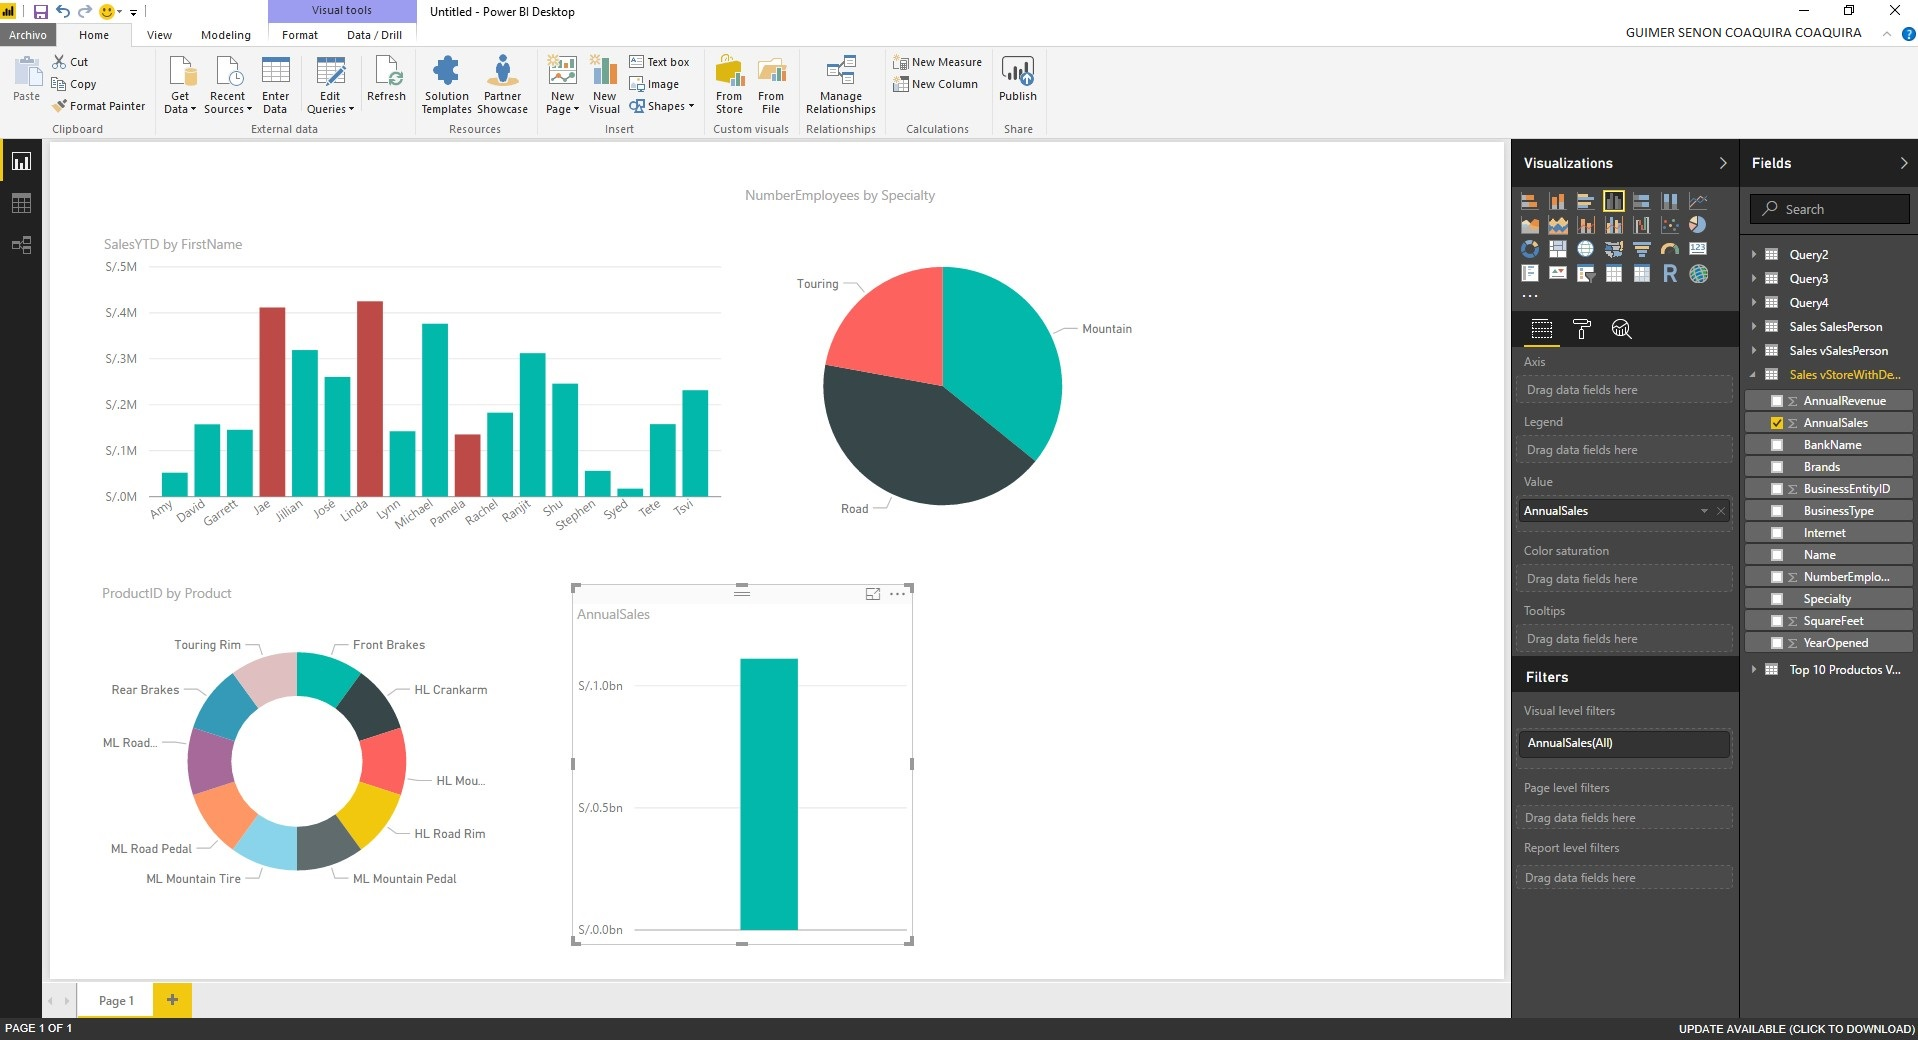
\includegraphics[width=15cm]{./Imagenes/Captura03}
\end{center}
\end{figure}

\subsection{RESULTADO Nº04:}
\begin{figure}[httb]
\begin{center}
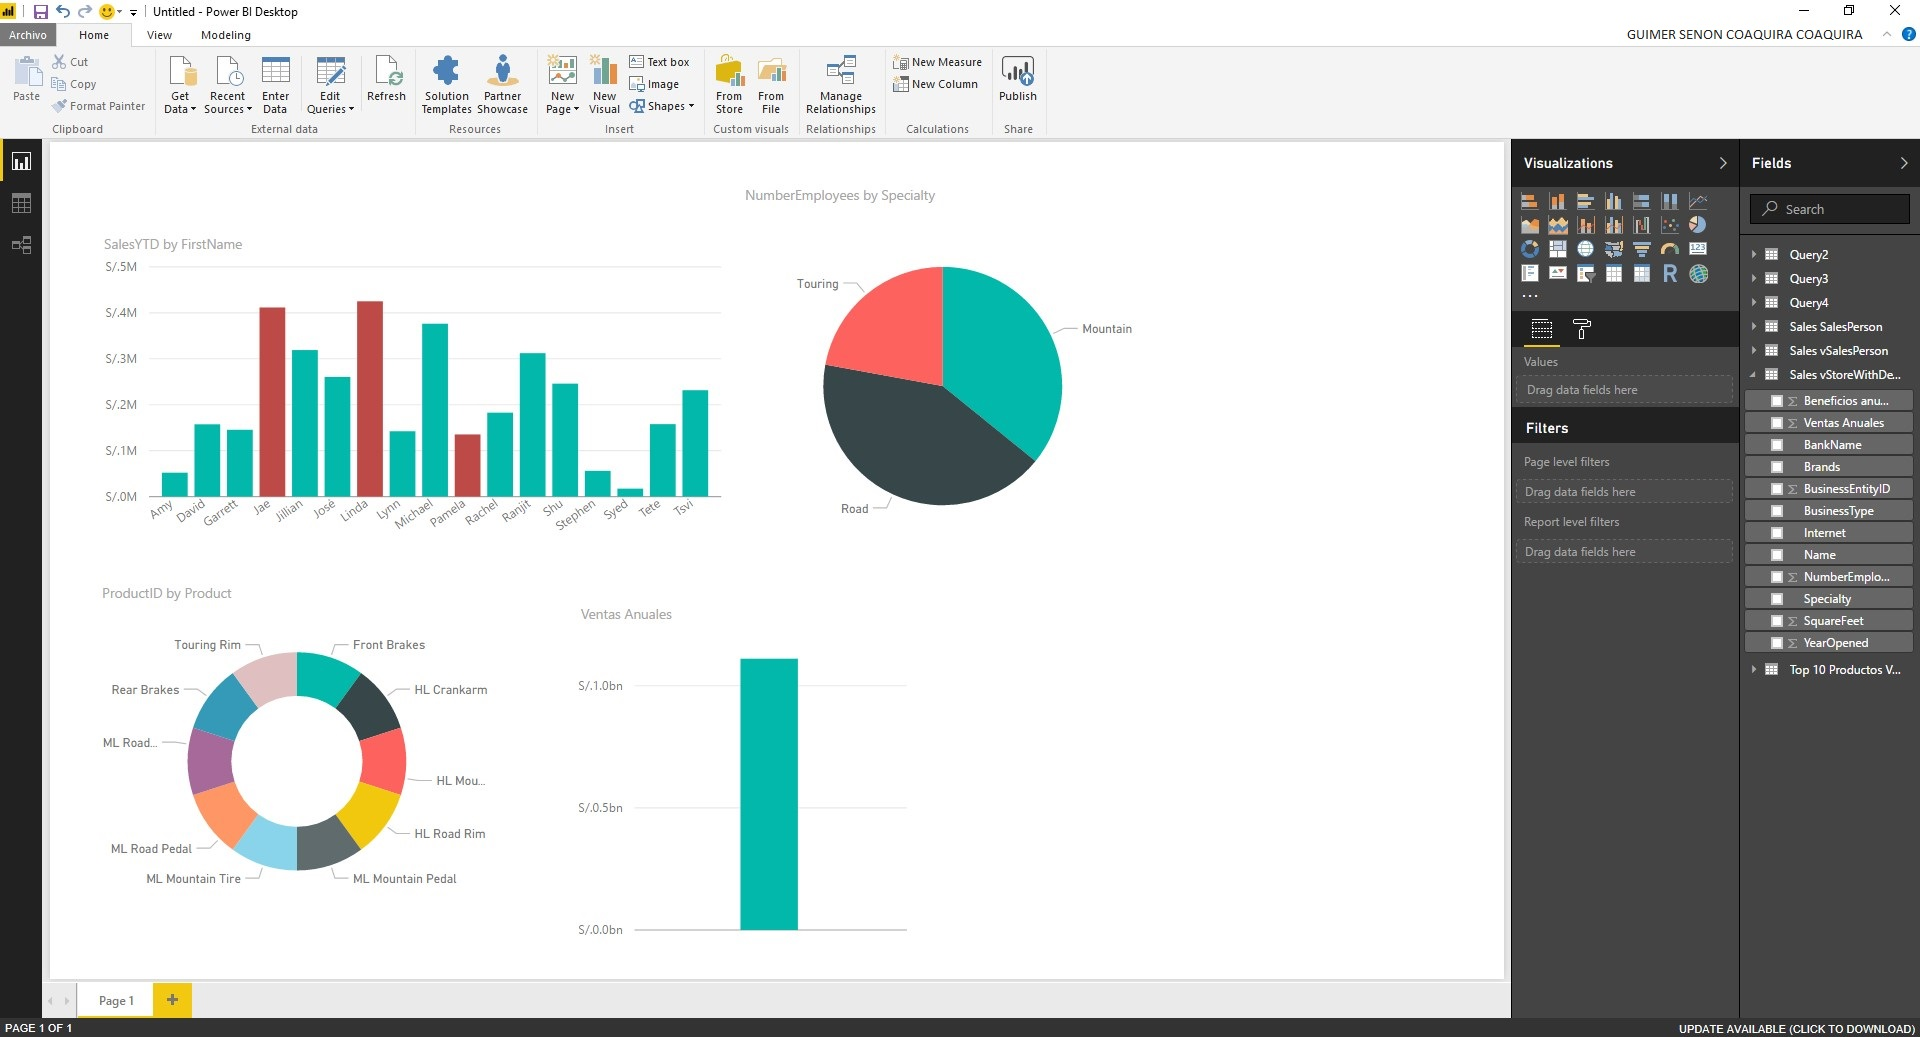
\includegraphics[width=15cm]{./Imagenes/Captura04}
\end{center}
\end{figure}
\newpage
\subsection{RESULTADO Nº05:}
\begin{figure}[httb]
\begin{center}
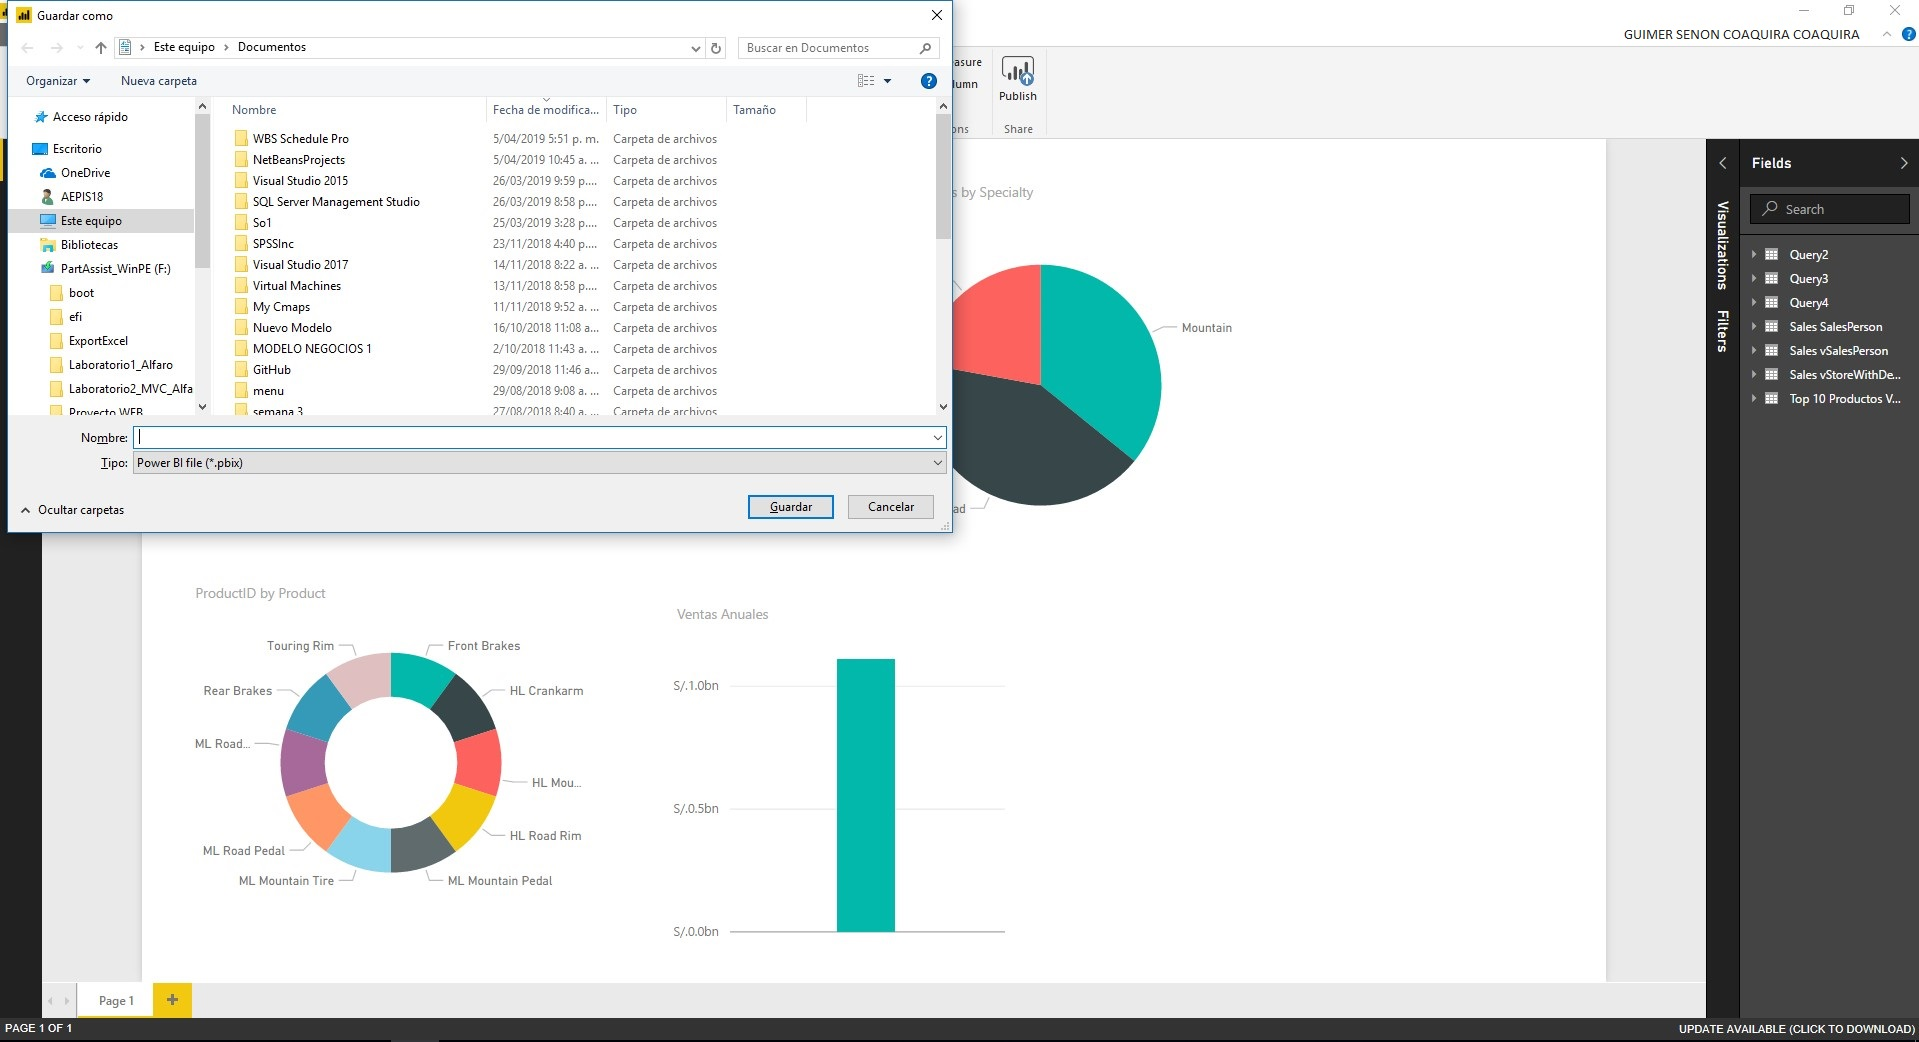
\includegraphics[width=15cm]{./Imagenes/Captura05}
\end{center}
\end{figure}

\subsection{RESULTADO Nº06:}
\begin{figure}[httb]
\begin{center}
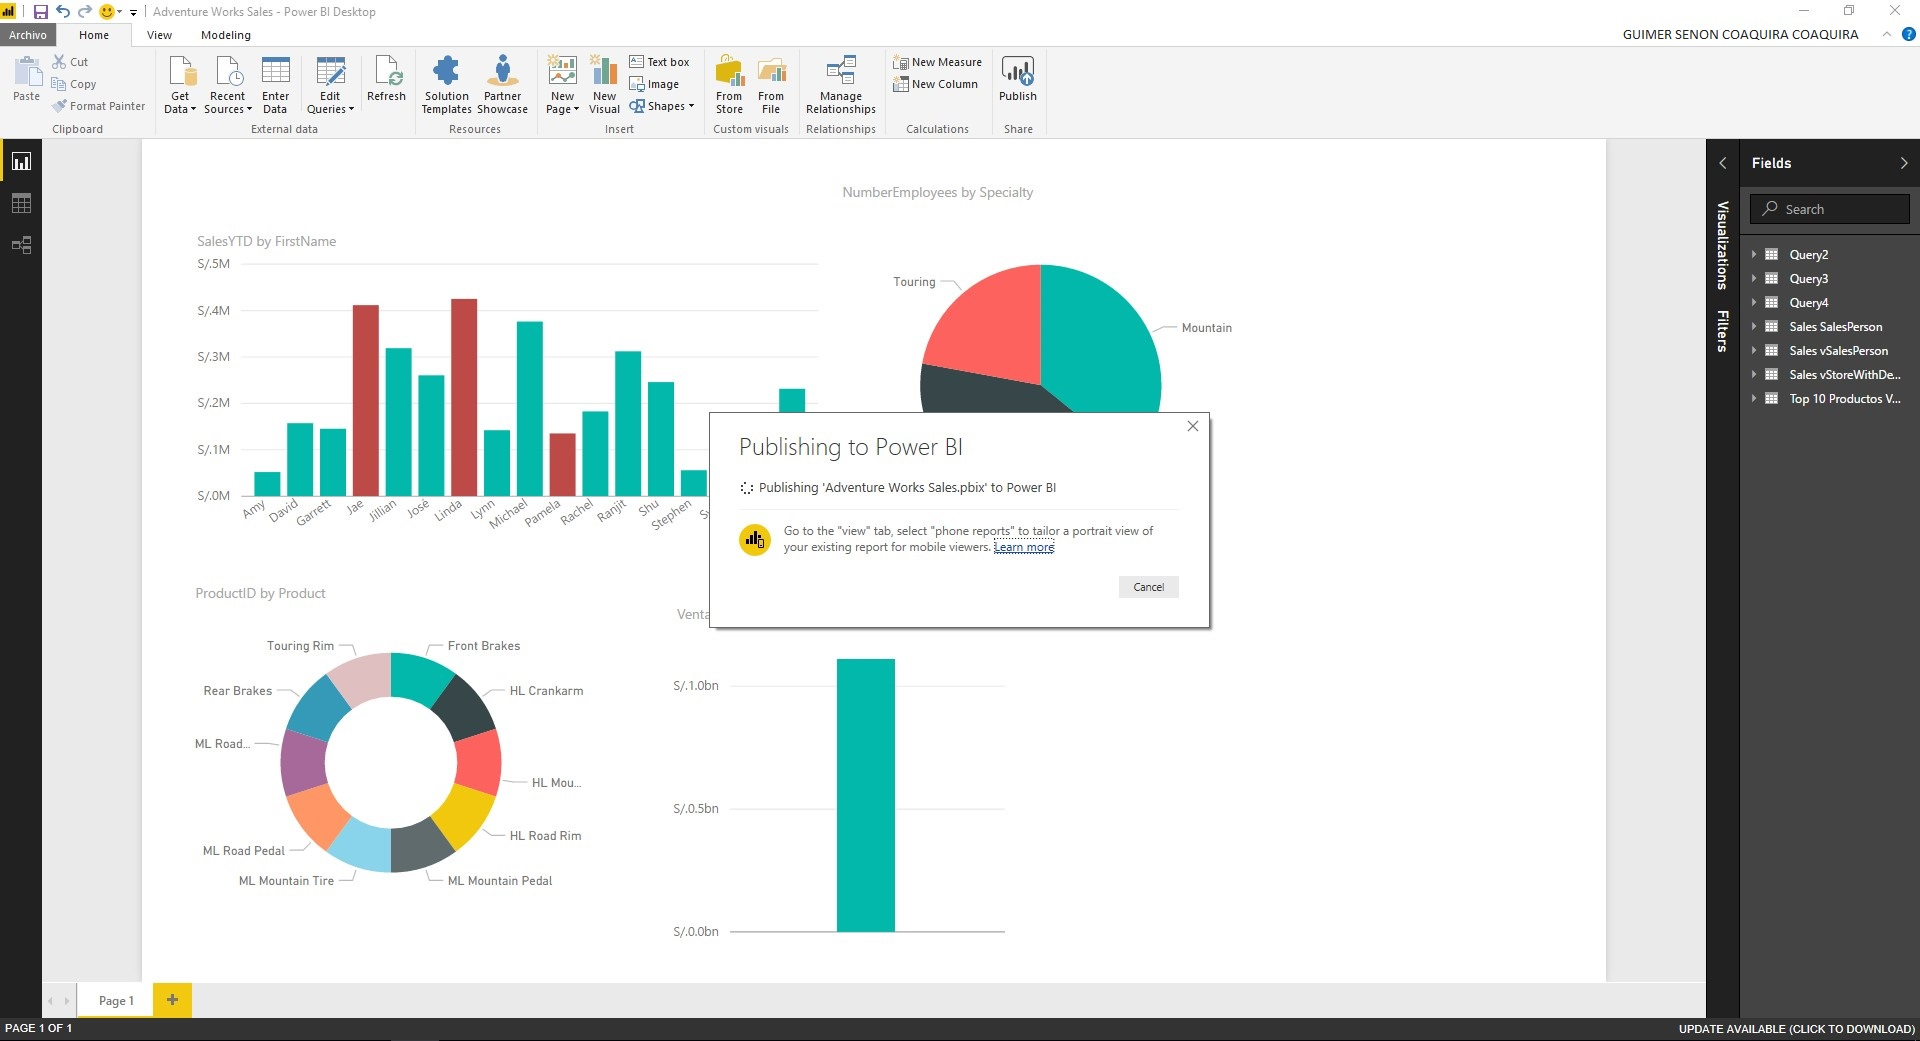
\includegraphics[width=15cm]{./Imagenes/Captura06}
\end{center}
\end{figure}
\include{Secciones/Actividad1}

\end{document}
